\chapter{Einleitung}

Ziel eines Teilchenbeschleuniger ist es einen Teilchenstrahl oder -bunch zu beschleunigen und m�glichst 
fokussiert auf einer Sollbahn zu halten. Einerseits um keine Teilchen zu verilieren, andersetits um z.B.
bei einem Collider die Teilchendichte hoch zu halten.
In unserem Versuch werden wir mit einem einfachen Linearbeschleuniger arbeiten und die Energie sowie die Emittanz,
eine die Qualit�t des Strahls charakterisierende Gr��e die wir im Theorieteil erkl�ren werden, zu messen.

\section{Aufbau}
\begin{figure}[ht]
  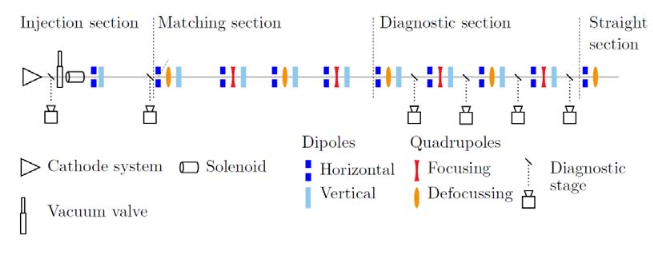
\includegraphics[width=0.8\textwidth]{./salome-aufbau.png}
  \caption{}
\end{figure}

Der Teilchenbeschleuniger vesteht aus einem Kathodenstrahler zur Erzeugung des Strahls, einer Spule 
(Solenoidmagnet) dessen �u�ere Streufelder fokussierend wirken, einigen Dipol- und Quadromagneten.
\begin{figure}[]
  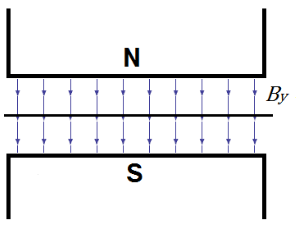
\includegraphics[width=0.40\textwidth]{./dipol.png}\hfill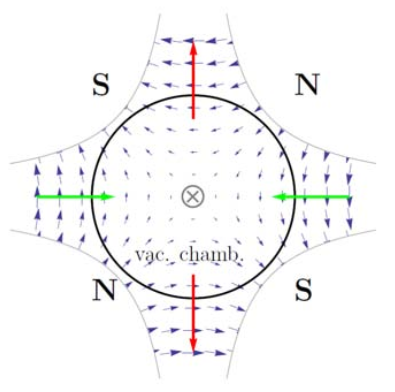
\includegraphics[width=0.40\textwidth]{./quadropol.png}
  \caption{Di-und Quadropolschemata}
  
\end{figure}
\newpage
Wie man im Bild xx illustriert sehen kann erzeugt der Dipolmagnet ein homogenes Magnetfeld in (vertikale) y-Richtung,
das daf�r geeignet ist externe Magnetfelder wie das Erdmagnetfeld zu kompensieren. 
Nehmen wir ein idealisierten Teilchenstrahl an, so lenkt  der Dipol den Strahl auf 
eine Kreisbahn e/p *By= 1/R.

P:Impuls in Richtung der Sollbahn

R:Raidus der Kreisbahn

Die St�rke des Dipols werden wir im Folgendem damit charakterisieren.
Der Quadropol h�ngt linear von x ab und wirkt in einer ebene fokussierend in der anderen defokussierend, 
deswegen werden sie um 90� gedreht hintereinander aufgebaut.

e/p*By(x)=kx

e/p*Bx(y)=-ky

k: St�rke des Quadropolmagneten

\newpage
\section{Theorie}
\section {Phasenraum, Emittanz und Twissparameter}
Man stellt zun�chst die Bewegungsgleichungen eines einzelnen Teilchens auf und guckt wie dieses sich unabh�ngig 
von den anderen Teilchen im Bezug auf die Sollbahn bewegt. Den Einfluss der Teilchen aufeinander kann hier 
vernachl�ssigt werden da der Strom sehr klein ist.
Hergeleitet findet man die DGL im Wille S. xx , die genaue Form soll uns hier aber nicht interessieren. Es stellt sich wie durch die fokussierende Wirkung der Quadropolmagnet 
vermutet heraus, dass ein Teilchen eine osillierende Bewegung um die Sollbahn durchf�hrt.

Im Phasenraum ist die Bewegung des Teilchens durch eine Ellipse beschrieben:

\begin{equation}
\epsilon=\gamma(s)x^2(s)+2\alpha(s)x(s)x'(s)+\beta(s)x'^2(s)\end{equation}

s soll hier die parametrisierung der Sollbahn darstellen.x(s) ist die Ablenkung zur Sollbahn, x'(s) Der Winkel zwischen Geschwindigkeit und Sollbahn. 

$\gamma(s),\alpha(s),\beta(s)$ sind die sogenannten ``Twissparameter'', sie bestimmten die Form und Position der Elllipse, und sind
auch abh�ngig von der Position auf der Sollbahn.
$\epsilon$ ist die Emittanz des Teilchens. Sie wurde als Integrationskonstante in den Bewegungsgleichungen eingef�hrt und ist daher unabh�ngig von s.
Sie ist bis auf den Faktor $\pi$ die Fl�che der Ellipse im Phasenraum.
  
